\chapter{Introduction of PitchApp}
\chapterauthor{by Boglarka Lehoczki}

PitchApp is intended to be a platform to help employees find the required organizational support to turn their ideas from inception to reality. The goal of our web application is, thus, to facilitate the launching of new projects. By making project ideas of colleagues easier and faster visible to management, PitchApp encourages employees to contribute more actively to the success of the company at which they work. In this way, PitchApp helps to achieve higher degrees of intrapreneurship, which leads to business growth. Using our application will bring companies ahead of the game, in terms of innovation and
employee engagement, as well as make big firms more competitive and flexible, thus more
profitable. Hence, “fast innovators take leadership positions in their industries” \parencite{SH90}.

PitchApp is a dynamic, single-page web application with database connection that we developed to enhance employee engagement and proactivity by connecting the employees’ ideas to even the highest levels of executives. Managers with budgets and resources for projects (i.e. potential future sponsors) can browse between different project ideas, which are posted by the employees. Distinct types of ideas are sorted into groups like HR, Procurement, R\&D etc., which facilitates searching among them. Then managers can offer their resources for the realization of a project idea, which they find valuable. Employees are also able to view the pitches posted by other colleagues in between their organization to avoid the sharing of redundant ideas. PitchApp is planned to be able to serve more large organizations at the same time and to be provided as a Software as a Service. PitchApp includes a user and session management system, which allows secure login and logout functionalities. It differentiates between public area, i.e. our landing page, and member area with two type of users, idea owners and idea sponsors.

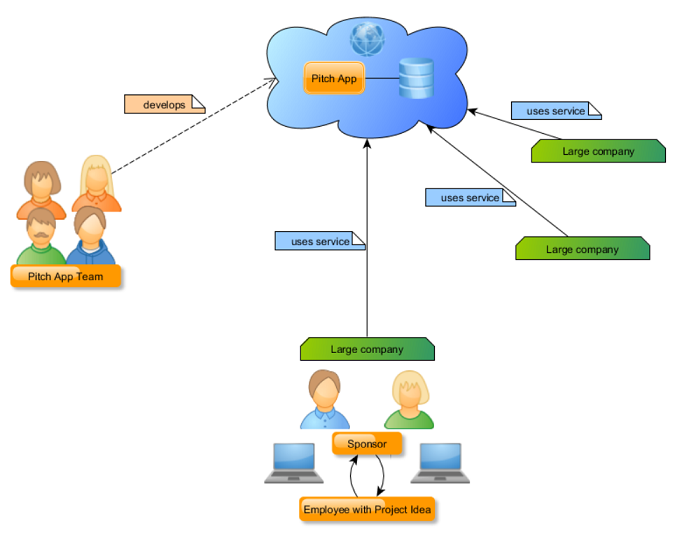
\includegraphics{pitchapp_saas.png}



\chapter{Architecture}
\chapterauthor{by Boglarka Lehoczki}
\chapter{Technologies used for Implementation}
\section{React and Reactstrap}
\chapterauthor{by Boglarka Lehoczki}
\section{Okta}
\chapter{Final Results}
\chapter{User Manual}
\chapter{Difficulties of Implementation}
\chapter{Future Outlook: Missing Components and Functionalities}



